\documentclass[12pt]{scrartcl}
\usepackage[sexy]{evan}
\usepackage{graphicx}

\usepackage{answers}
\Newassociation{hint}{hintitem}{all-hints}
\renewcommand{\solutionextension}{out}
\renewenvironment{hintitem}[1]{\item[\bfseries #1.]}{}
\declaretheorem[style=thmbluebox,name={Theorem}]{thm}

 %Sets
\newcommand{\N}{\mathbb{N}}
\newcommand{\Z}{\mathbb{Z}}
\newcommand{\F}{\mathbb{F}}
\newcommand{\Q}{\mathbb{Q}}
\newcommand{\R}{\mathbb{R}}
\newcommand{\C}{\mathbb C}
\newcommand{\D}{\mathbb D}

\newcommand{\T}{\mathbb T}
\renewcommand{\hat}{\widehat}
\renewcommand{\tilde}{\widetilde}

\let \phi \varphi
\let \mc \mathcal
\let \ol \overline
%From Topology
\newcommand{\cT}{\mathcal{T}}
\newcommand{\cB}{\mathcal{B}}
\newcommand{\cC}{\mathcal{C}}
\newcommand{\cH}{\mathcal{H}}

\newcommand{\supp}{\text{supp }}

\newcommand{\aint}{\mathrel{\int\!\!\!\!\!\!-}}
\let \grad \nabla

\begin{document}
\title{Math 205}
\author{Vishal Raman}
\thispagestyle{empty}
$ $
\vfill
\begin{center}

\centerline{\huge \textbf{Math 205: Complex Variables} } 
\centerline{Professor: Dan-Virgil Voiculescu, Spring 2021}
\centerline{Scribe: Vishal Raman}
\end{center}
\vfill
$ $
\newpage
\thispagestyle{empty}
\tableofcontents
\newpage
%\maketitle
\section{January 20th, 2021}
\subsection{Intro to Riemann Mapping Theorem}
Our first goal is to proof a fundamental theorem of Riemann on conformal mappings.  We start with several preparations, including some detours.  The theorem essentially says that lots of open sets in $\C$ are holomorphically isomorhpic, given that they satisfy some simple topological conditions.  

\subsection{Cauchy's Integral Formula}
Recall Cauchy's formula:
$$f(z_0) = \frac{1}{2\pi i} \int_{\Gamma} \frac{f(z)}{z - z_0} \,dz$$
where $\Gamma$ is a simple closed curve, piecewise differentiable, $z_0 \in \text{Int}(\Gamma)$, and $f : \Omega \to \C$ is a holomorphic function, with $\Omega$ is open, $\Omega \supset \Gamma \cup \text{Int}(\Gamma)$.

If $\Gamma$ is the circle $|z - z_0| = R$, we parameterize with $z = Re^{i\theta} + z_0$ with $\theta \in [0, 2\pi)$.  This gives
$$f(z_0) = \frac{1}{2\pi} \int_{0}^{2\pi} f(z_0 + Re^{i\theta})\,d\theta,$$
which represents the average of $f$ on the circle.  

It follows that 
$$|f(z_0)| \le \max_{\partial B_R(z_0)} |f(z)|,$$
with equality if and only if $f$ is constant.  

If $f: \Omega \to \C$ is holomorphic for $\Omega$ connected, open and $z_0 \in \Omega$, then
$$|f(z_0)|\le \sup_{z \in \Omega} |f(z)|$$
with equality if and only if $f$ is constant.  

\subsection{Schwarz Lemma}
 \begin{thm}[Schwarz Lemma] For $f: B_1(0) \to \C$ holomorphic with $|f(z)|\le 1$ for all $z$ and $f(0) = 0$.  Then
 $$|f(z)| \le |z|, |f'(0)| \le 1.$$
 If for some $z_0 \ne 0$, $|f(z_0)| = |z_0|$ or if $|f'(0)| = 1$ then $f(z) = cz$ for some $|c| = 1$.
 \end{thm}
 \begin{proof}
 Define a function
 $$g(z) = \begin{cases} f(z)/z, \text{if } 0 \le |z| \le 1 \\
 f'(0), \text{if } z = 0
 \end{cases}.$$
 
 Note that $g(z)$ is continuous since at zero,
 $$\lim_{z \to 0} \frac{f(z)}{z} = \lim_{z \to 0} \frac{f(z) - f(0)}{z - 0} = f'(0).$$
 
 Hence, $|g(z)| \le C < \infty$ using the Weierstrass Extreme Value theorem.    If $0 < \epsilon < |w| < r < 1$, note that taking a Keyhole Contour, we have
 $$g(w) = \frac{1}{2\pi i} \left (\int_{|z| = r} - \int_{|z| = \epsilon}\right ) \frac{g(z)}{z - w}\,dz.$$
 
Note that
 $$\left |\int_{|z| = \epsilon} \frac{g(z)}{z-w}\,dz\right | \le (2 \pi \epsilon) \cdot C \frac{1}{|w| - \epsilon} \xrightarrow{\epsilon \to 0} 0.$$
 
 It follows that $$g(w) = \frac{1}{2\pi i} \int_{|z| = r} \frac{g(z)}{z - w}\, dz$$
 for $0 < |w| < r$.  The right side is holomorphic in $w$ if $|w| < r$, so it follows that 
 $$g(w) = \frac{1}{2\pi i} \int_{|z| = r} \frac{g(z)}{z - w}\, dz$$
 is holomorphic in $|z| < 1$.  
 
 This can also be proved by taking a Taylor series about the origin.  Since there is no constant term, we can divide by $z$ to still have a convergent Taylor series.  
 
 If $r < 1$,
 $$\sup_{|z| \le r} |g(z)| = \sup_{|z| = r} |g(z)| \le \sup_{|z| = r} \frac{|f(z)|}{|z|} \le \frac{1}{r}.$$
 
 If we let $r \uparrow 1$, then we get $\sup_{|z| < 1} |g(z) |\le 1$.  It follows that $|f(z)| \le |z|,$ $|f'(0)| \le 1$.
 
 If $|f(z_0)| = z_0$ for some $0 < |z_0| < 1$ then $|g(z_0)| = 1$ and $g$ is constant by the maximum principle so $g(z) = c$, $f(z) = cz$.  If $|f'(0)| = 1$, then $|g(0)| = 1$ so $g$ is constant and $f = cz$.
 \end{proof}
\subsection{Maximum Principles} 
In the above proof, we used the maximum principle.  Some other versions we will use are the following:
 
 If $K \subset \C$ compact and $f:K \to \C$ continuous, and the restriction of $f$ to the interior of $K$ is holomorphic, then 
 $$\sup_{z \in K} |f(z)| = \sup_{z \in \partial K} |f(z)|.$$
 
If $\Omega$ is open and connected, $f: \Omega \to \C$, $z_0 \in \Omega$, and $|f(z_0)| = \sup_{z \in \Omega} |f(z)|$, then $f$ is constant.  Applying this to $e^f$ and using that $|e^f| = e^{\text{Re }f}$, we find that 
$$\text{Re }f(z_0) = \sup_{z \in \Omega} \text{Re }f(z),$$
implies that $f$
 is constant.   We have the same result for $\text{Im }f$ by replacing $f$ with $-if$.  
 
% \subsection{Homework I }
%Show the Automorphisms of the unit disk are fractional linear transformations.
%\begin{proof}
%Following the hint, define $h = g \circ f$.  Note that $h: \{|z| < 1\} \to \{|z| < 1\}$ is a holomorphic bijection as a composition of holomorphic bijections.  Furthermore, note that $$h(0) = \frac{f(0) - z_0}{1 - \ol{z_0} f(0)} = \frac{z_0 - z_0}{1 - \ol{z_0} f(0)} = 0.$$
%
%Note that we can apply the Schwarz lemma to $h$ and $h^{-1}$ since the ranges of both functions are $\{|z| < 1\}$.  It follows that $|h'(0)| \le 1$ and 
%$$1 \ge |(h^{-1})'(0)| = \left |\frac{1}{h'(h^{-1}(0))}\right | = \left |\frac{1}{h'(0)}\right |.$$
%It follows that $|h'(0)| = 1$, so by the equality case of the Schwarz lemma, $h(z) = cz$ for some $c \in \C$.
%
%It follows that $$h(z) = \frac{f(z) -z_0}{1 - \ol{z_0} f(z)} = cz \Rightarrow f(z) = \frac{z_0 + cz}{1 + c\ol{z_0}z} = \frac{a + bz}{c + dz}$$
%for $a, b, c, d \in \C$.
%\end{proof}
\pagebreak
\section{January 25th, 2021}
\subsection{Uniform Convergence}
\begin{remark} They sometimes call open connected sets "regions".
\end{remark}

\begin{definition}[Uniform Convergence] Let $\Omega \subset \C$ be open.  Let $f_n: \Omega \to \C$ be holomorphic and $f: \Omega \to \C$ a function so that $\lim_{n \to \infty} \sup_{z \in K} |f(z) - f_n(z)| = 0$ for all $K \subset \Omega$ compact(also denoted $K \subset \subset \Omega$).  
\end{definition}
\begin{remark} Recall from real analysis that $f$ is a continuous function.  
\end{remark}

Some further remarks:
\begin{itemize}
\item It suffices to check the result for a sequence of compact subsets $K_m$ so that $\bigcup_m K_m^\circ = \Omega$, the it suffices to check those.  If $K \subset \subset \Omega$, then $K$ is compact and covered by the union of the subsets so there exists a finite subcovering, and uniform convergence on the subcovering implies uniform convergence on $K$.
\item It is often convenient to introduce $\|g\|_K = \sup_{z \in K} |g(z)|$.  Uniform convergence can be restated as $\|f_n - f\|_K \to 0$ for all $K \subset \subset \Omega$.
\item If $\|f_n - f\|_K \to 0$ for all $K \subset \subset \Omega$, then $f$ is also holomorphic.  It follows by passing to the limit in the Cauchy Integral formula.  Namely, take $\{z : |z - z_0| \le R\} \subset \Omega$ and consider the points in $|z_0 - \zeta| < R$.  

\begin{align*}
\left |f_n(\zeta) - \frac{1}{2\pi i} \int_{|z - z_0| = R} \frac{f(z)}{z - \zeta}\,dz\right | &= \left |  \frac{1}{2\pi i} \int_{|z - z_0| = R} \frac{f_n(z)}{z - \zeta}\,dz  - \frac{1}{2\pi i} \int_{|z - z_0| = R} \frac{f(z)}{z - \zeta}\,dz\right | \\
&\le \frac{1}{2\pi} \frac{1}{R - |z_0 - \zeta|} \cdot (2\pi R) \|f_n - f\|_{|z - z_0| = R} \to 0.
\end{align*}
So it follows that 
$$f(\zeta) = \lim_{n \to \infty} f_n(\zeta) = \frac{1}{2\pi i} \int_{|z - z_0|} \frac{f(z)}{z - \zeta} \,dz.$$

It follows that $f$ continuous on $|z - z_0| = R$ is holomorphic in $\zeta\in \{|z - z_0| < R\}$, so it follows that $f$ is holomorphic.  
\item We can similarly show that 
$$f_n^(j)(\zeta) = \frac{n!}{2\pi i} \int_{|z - z_0| = R} \frac{f_n(z)}{(z - \zeta)^{n+1}}\,dz$$
and $\|f_n^{(j)} - f^(j)\|_K \to 0$.  
\end{itemize}
From the last item, we have the following theorem.
\begin{thm} If $f_n \to f$ on compact subsets of $\Omega$, the if $f_n$ is holomorphic we find that $f$ is holomorphic and $f_n^(j) \to f^{(j)}$ uniformly on compact subsets of $\Omega$.
\end{thm}

\begin{thm}[Hurwitz] Let $\Omega$ be a region, $f : \Omega \to \C$ and $f_n: \Omega \to \C$ holomorphic with $f_n(\Omega) \subset \C \setminus \{0\}$, $n \in \N$ and $\|f_n - f\|_K \to 0$
 for all compact subsets.  Then either $f \equiv 0$ or $f(\Omega) \subset \C \setminus \{0\}$.
 \end{thm}
\begin{proof}
If $f$ is not identically zero on $\omega$, then since $f$ is holomorphic, its zeros are isolated.  If $z_0 \in \Omega$, $f(z_0) = 0$, then there is $\epsilon > 0$ so that when $0 < |z - z_0| <\epsilon$, $f(z) \ne 0$. 

Since $f(z) \ne 0$ for $|z - z_0| = \epsilon/2$, by the Weierstrass theorem applied to $|f|$ on $|z - z_0| = \epsilon$, we have $|f(z)| \ge m > 0$ on $\{|z - z_0| = \epsilon/2\} = \Gamma$.  If $\|f_n - f\|_\Gamma \le m/2$ for $n \ge N$, then $$|f_n(z)| \ge |f(z)| - m/2 \ge m - m/2 = m/2$$ for $z \in \Gamma$.  Hence, it follows that $\|1 /f_n - 1/f\|_\Gamma \to 0$(we leave this as an exercise).

Since $\|f_n' - f'\|_\Gamma \to 0$, we find that $\|f_n'/f_n - f'/f\| \to 0$(another exercise) and hence
$$\frac{1}{2\pi i} \int_\Gamma \frac{f_n'}{f_n}\,dz \to \frac{1}{2\pi i}\int_\Gamma \frac{f'}{f}\,dz.$$
The integrand of the left hand side is $(\log f_n)'$, whose integral is $0$, and the right side is the order of the zero of $f$ at $z_0$ by the argument principle.    It follows that the order of $z_0$ as a possible zero is $0$, so $f(z_0) \ne 0$.
\end{proof}

\begin{thm} For $\Omega \subset \C$ open, $\mc F$
 a set of holomorphic functions, the following are equivalent:
 \begin{itemize}
 \item for every $K \subset \subset \Omega$ $\sup_{f \in \mc F} \|f\|_K < \infty$
 \item for every sequence $(f_n)_{n \in \N} \subset \mc F$, there is a subsequence $(f_{n_j})_{j \in \N}$ with $n_1 < n_2 < \dots$ so that $(f_{n_j})_{j \in \N}$ is uniformly convergent on compact subsets of $\Omega$.
 \end{itemize}
 \end{thm}
 \begin{proof}
 We first show $2$ implies $1$.  If $\sup_{f \in \mc F} \|f\|_K = \infty$, then we can find for each $n \in \N$ $f_n \in \mc F$ so that $\|f_n\|_K \ge n.$  If we abstract a convergence subsequence, then $\|f_{n_j} - f\|_K \le C < \infty$ and $\|f_{n_j}\|_K \le \|f\|_K + C$, while $\|f_{n_j}\|_K \to \infty$, a contradiction.
 \end{proof}
 \pagebreak
 \section{January 27th, 2021}
 \subsection{Uniform Convergence, continued}
 \begin{thm} For $\Omega \subset \C$ open, $\mc F$
 a set of holomorphic functions, the following are equivalent:
 \begin{itemize}
 \item for every $K \subset \subset \Omega$ $\sup_{f \in \mc F} \|f\|_K < \infty$
 \item for every sequence $(f_n)_{n \in \N} \subset \mc F$, there is a subsequence $(f_{n_j})_{j \in \N}$ with $n_1 < n_2 < \dots$ so that $(f_{n_j})_{j \in \N}$ is uniformly convergent on compact subsets of $\Omega$.
 \end{itemize}
 \end{thm}
 I missed the beginning of the class, but I will add the proof of the theorem once notes are posted.
 \subsection{Metric Convergence}
 One can put a metric on holomorphic functions so that convergence in the metric is uniform convergence on compact sets.  For $f: \Omega \to \C$, but $K_n \Subset \Omega$ so that $\bigcup_{n} K_n^\circ = \Omega$ and take 
 $$d(f, g) = \sum_{n=1}^\infty \frac{\|f - g\|_{K_n}}{1 + \|f - g\|_{K_n}} 2^{-n}.$$
 
 \subsection{Riemann Sphere}
 On the set $\C \cup \{\infty\}$, we consider the topology which makes it the Alexandroff(one-point) compactification of $\C$.  If $z \in \C$, a neighborhood is one that contains a neighborhood in $\C$ and a neighborhood of $\infty$
 is of the form $\{\infty\} \cup (\C \setminus K)$ for $K \Subset \C$.
 
Let $U_+ = \C \subset \C \cup \{\infty\}$ and $U_- = (C \setminus \{0\}) \cup \{\infty\}$.  Note that the union of the two sets covers the Riemann Sphere.  Define $\psi_+:U_+ \to \C$ by $\psi_+(z) = z$ and $\psi_i: U_- \to \C$ is given by $\psi_-(w) = 1/w$ if $w \in \C \setminus \{\infty\}$ and $0$ if $w = \infty$.  Notice that these two functions are bijections.

If $V \subset \C \cup \{\infty\}$ is open, a function $f: V \to \C$ is holomorphic if 
$$f \vert_{V \cup U_\pm}\circ (\psi_{\pm}\vert_{V \cup U_\pm})^{-1}: \psi_\pm(V \cup U_\pm) \to \C$$
is holomorphic.  In this way, we know what holomorphic functions are on open sets of $\C \cup \{\infty\}$.

More generally, we can describe a Riemann surface in the following way - Let $X$ be a topological space.  Take $\{(U_\alpha, z_\alpha)\}_{\alpha \in I}$ where $U_\alpha \subset X$ is open, and $\bigcup_{\alpha \in I} U_\alpha = X$ and $z_\alpha: U_\alpha \to \C$ is continuous, $z_\alpha(U_\alpha)$ is open and $z_\alpha$ is a homeomorphism.  The key requirement is that the maps $z_\alpha \circ z_\beta^{-1}: z_\beta(U_\alpha \cup U_\beta) \to z_\alpha(U_\alpha \cup U_\beta)$ are holomorphic.

Then, if $U \subset X$ is open, $f: U \to \C$ is holomorphic if for all $\alpha \in I$,
$$f\vert_{U \cup U_\alpha} \circ (z_\alpha \vert_{u \cup U_\alpha})^{-1}$$
is holomorphic.  Two such atlases give the same Riemann surface if put together, we get an atlas.
\pagebreak
\section{February 1st, 2021}
\subsection{Connectivity}
\begin{definition} $\Omega\subset \C$ open is connected if $\Omega = \Omega_1 \cup \Omega_2$ open with $\Omega_1 \cap \Omega_2 = \emptyset$ implies that one of the two is empty.  For open sets, this is equivalent to arcwise connected.
\end{definition}


\begin{definition} An set is arcwise connected if for every $z_1, z_2 \in \Omega$, there is a path $\phi: [0, 1] \to \Omega$ which is continuous and $\phi(0) = z_1$, $\phi(1) = z_2$.
\end{definition}

\begin{definition} $\Omega$ is simply connected if for $z_0 \in \Omega$, $\Gamma:[0, 1] \to \Omega$
 continuous and $\Gamma(0) = \Gamma(1) = z_0$, then there is $G:[0, 1] \times [0, 1] \to \Omega$ continuous with $G(t, 0) = \Gamma(t)$ for $t \in [0, 1]$ and $G(t, 1) = z_0$, for $t \in [0, 1]$.  
 \end{definition}
 
 Simply connected corresponds to the idea of being able to continuously deform the set to a point for each point.
 
In $\R^2 \cong \C$, $\Omega$-open simply connected is equivalent to $(C \cup \{\infty\}) \setminus \Omega$ is connected in $\C \cup \{\infty\}$.  That is, if $F = \C\cup\{\infty\} \setminus \Omega$, which is closed in $\C \cup \{\infty\}$, with $F \cap V_1 \cap V_2 = \emptyset$, then at least one of the $F \cap V_k = \emptyset$.  If $0 \in \Omega$, then $\Omega$ is simply connected if and only if $\{0\} \cup \{1/z : z \in \C \setminus \Omega\}$ is connected(this is a local representation).

\begin{itemize}
\item Take $\Omega = \C \setminus \bigcup_{j=1}^m \{tz_j : t \in [1, \infty)\}$ for $z_1, \dots, z_n \in \C \setminus \{0\}$.  
\item $\C \setminus\text{spirals}$.
\end{itemize}

\begin{thm}[Riemann Mapping Theorem] If $\Omega \subset \C$ open, connected, simply connected, $\emptyset \ne \Omega \ne \C$, then $\Omega$ and $\mathbb{D} = \{|z| < 1\}$ are holomorphic isomorphisms.  
\end{thm}

\subsection{Fractional Linear Transformations}
Recall that if $f \in \text{Aut}(\mathbb D)$ then $f(z) = \frac{az+b}{xz + d}$, which was proved using the Schwarz lemma.  We view the fractional linear maps from a different context.  

We define a map $p: \C^2 \setminus\{\binom{0}{0}\} \to \C \cup \{\infty\}$ given by 
$$p\left (\binom{z_1}{z_2}\right ) = \begin{cases}
z_1/z_2 \text{ if }z_2 \ne 0\\
\infty \text{ if } z_2 = 0
\end{cases}.$$

Then $p(\xi) = p(\eta)$ if and only if $\xi = \lambda \eta$ for $\lambda \in C^\times = C \setminus \{0\}$.  

There is a larger group acting on $C^2 \setminus \{\binom{0}{0}\}$ given by $GL(2, \C)$ the invertible $2 \times 2$ matrices in the natural way so that $$A\binom{z_1}{z_2} \mapsto \frac{A_{11} p(\xi) + A_{12}}{A_{21}p(\xi) + A_{22}}.$$

Define $T_g: \C \cup \{\infty\} \to \C \cup \{\infty\}$ given by 
$$T_g z = \frac{az+b}{cz+d},$$
with $T_g (\infty )= \frac{a}{c}$.  We have the action $T_gp(\xi) = p(g\xi)$ for $g \in GL(2, \C)$.  

This gives 
$$T_{g_1} \circ T_{g_2} = T_{g_1g_2},$$
$$(T_g)^{-1} = T_{g^{-1}}.$$
 
We can also ask about the fixed point: $$T_gp(\xi) = p(\xi) \leftrightarrow p(\xi) = p(g\xi) \Leftrightarrow
 g\xi = \lambda \xi\,\, ,\lambda \in C^\times$$
 It follows that the fixed points of $T_g$ correspond to the eigenvectors of $GL(2, \C)$.
 
\subsection{Fractional Linear Transformations, Unit Disk}
If we have $\xi = \binom{z_1}{z_2}$, then $p(\xi) \in \mathbb D$ if and only if $|z_1| < |z_2|$ if and only if $z_1 \ol{z_1} - z_2 \ol{z_2} < 0$.  If we let $$J = \begin{pmatrix}
1, 0\\
0, -1
\end{pmatrix},$$
we consider the sesquilinear form $\langle J\binom{\xi_1}{\xi_2}, \binom{\eta_1}{\eta_2}\rangle$, where it is linear in the first coordinate and conjugate linear in the second coordinate.  Note that 

$$\langle J\binom{\xi_1}{\xi_2}, \binom{\eta_1}{\eta_2}\rangle = \xi_1 \ol{\eta_1} - \xi_2 \ol{\eta_2}.$$

When does $g \in GL(2, \C)$ preserve $\langle J\xi, \xi\rangle$?

This means that 
$$\langle Jg\xi, g\xi \rangle = \langle J\xi, \xi \rangle$$
for all $\xi \in C^2 \setminus \{0\}$.  Then,
$$\langle g^* Jg \xi, \xi\rangle = \langle J\xi, \xi\rangle$$
so it follows that $g^*Jg = J$.  (We prove this by transforming $\xi$ in polar coordinates, $\xi = x + i^k y$, and considering $k = 0, 1, 2, 3$.  These four equations allow us to determine the equality).  Note that $U(1, 1) = \{g : g^* J g = J\}$ forms a group structure where $J$ has eigenvalues $\pm 1$  for this reason, we denote $U(1, 1) \subset GL_2(\C)$.

We claim the following: $T_g \in \text{Aut}(\mathbb D) \Leftrightarrow g \in C^\times \cdot U(1, 1)$.
%\subsection{Homework II}
%Show that the series $\zeta(z) = \sum_{n=1}^\infty n^{-z}$ converges uniformly on compact subsets of $\{z \in \C : \text{Re}(z) > 1\}$.
%\begin{proof}
%Let $D \subset \subset \{z \in \C : \text{Re}(z) > 1\}$.  Note that $D \subset H = \{z \in \C : \text{Re}(z) \ge c\}$ for some $c > 1$, so it suffices to show that the series is uniformly convergent on $H$.  
%
%Note that $$|n^{-z}| = |e^{-z \log n}| |e^{-\text{Re}(z)\log n - i\text{Im}(z) \log n}| = e^{-\text{Re}(z)\log n}| \le |e^{-c\log n}| = n^{-c}.$$
%
%Note that $\sum_{n=1}^{\infty} n^{-c} < \infty$ since $c > 1$, so it follows that $\zeta(z)$ converges uniformly on $H$ (and hence $D$) by the Weierstrass M-test.
%\end{proof}

\pagebreak
\section{February 3rd, 2021}
\subsection{Remark on the Zeta Function}
\begin{theorem}[S.M. Voronin 1975] For $D = \{\frac{1}{2} < \text{Re}(z) < 1\}$, $f : D \to \C \setminus \{0\}$.  If $K \subset \subset D$ and $\epsilon > 0$, then there exists $t \in \R$ such that 
$$\|f(\cdot) - \zeta(\cdot + it) \|_K < \epsilon.$$
\end{theorem}

This theorem essentially says that if I slide around the zeta function in the strip $D$, I can uniformly approximate pretty much any function I want.  

\subsection{Fractional Linear Transformations, continued}
Note that $\text{Ker}(g \mapsto T_g) = C^\times I_2$.  We define $SL(2; C) = \{g \in GL(2; \C) : \det g = 1\}$, the special linear group.  

\begin{theorem} For $g \in SL(2; C)$, $T_g \in \text{Aut}(\mathbb D)$ if and only if $g \in U(1, 1)$.
\end{theorem}
\begin{proof}
We start with the forward direction.  From the first homework, we showed that $f \in \text{Aut}(\mathbb D)$ implies that $f(z) = T_g z$ where $g$ is the composition of a rotation $g_1$ and $g_2 = \begin{pmatrix}
1 & z_0 \\
\ol{z_0} & 1
\end{pmatrix}$ for $z_0 \in \mathbb D$.  It suffices to check that $g_1, g_2 \in U(1, 1) \times \C^\times I_2$.  This is easy to check.  

Now, we show the converse.  If $g \in U(1, 1)$, then $g^{-1} \in U(1, 1)$.  If $z \in \mathbb D$, then $z = p(\xi), \langle J\xi, \xi\rangle < 0$.  We have $T_gz = p(g\ xi)$ and $\langle J\xi, \xi \rangle < 0$ implies that $\langle g^* j g\xi, \xi \rangle < 0$, which implies that $\langle Jg \xi, g\xi \rangle < 0$, which shows that $T_g z = p(g\xi) \in \mathbb D$.  Hence $T_g \mathbb D \subset \mathbb D$.  The same argument holds for $T_g^{-1} \mathbb D \subset \mathbb D$  so we have $T_g \mathbb D = \mathbb D$ exactly, so $T_g = \text{Aut}(\mathbb D)$.
\end{proof}

\subsection{Automorphisms of the Half Plane}
There is a conformal map from $\mathbb H_+ \to \mathbb D$ given by $f: z \mapsto \frac{z-i}{z+i}$.  This corresponds to $$f = \begin{pmatrix}
1 & -i \\
1 & i
\end{pmatrix}.$$  Note that $$f^{-1} = \frac{1}{2}\begin{pmatrix}
1 & 1 \\
i & -i
\end{pmatrix}.$$

Now, $\text{Aut}(\mathbb H_+) = \{(T_f)^{-1} T_g T_f | T_g \in \text{Aut}(\mathbb D)\} = \{T_{f^{-1}g f} | g \in SU(1, 1)\}$.  it follows that $\text{Aut}(\mathbb H_+) = \{T_h | f h f^{-1} \in SU(1, 1)\}$(assuming $h \in SL(2, \C)$, $fhf^{-1} \in SL(2, \C)$).  It follows that $(fhf^{-1})^* J (fhf^{-1}) = J$, so $h^* (f^* J f) h = f^* J f$.  We can compute $$f^* J f =  \begin{pmatrix}
0 & -2i \\
2i & 0  
\end{pmatrix}.$$ 

It follows that 
$$h^* \begin{pmatrix}
0 & -1 \\
1 & 0  
\end{pmatrix}h = \begin{pmatrix}
0 & -1 \\
1 & 0  
\end{pmatrix}.$$

If we let $h = \begin{pmatrix}
a & b \\
c & d 
\end{pmatrix}$,
then 
$$\begin{pmatrix}
0 & -1 \\
1 & 0  
\end{pmatrix} h^* \begin{pmatrix}
0 & -1 \\
1 & 0  
\end{pmatrix} h = I_2.$$

If we check the computation, we find that $a, b, c, d \in \R$, so it follows that $h \in SL(2, \R)$. 

\subsection{The Cross Ratio}
Note that $T_g$ is completely determined by $T_g 0, T_g 1, T_g \infty$.   Suppose $T_g 0 = T_h 0$, $T_g 1 =T_h 1$, $T_g\infty = T_h \infty$.  If we let $r = g^{-1} h$, we have $T_r 0 = 0, T_r 1 = 1, T_r \infty = \infty$, so it follows that $r \in C^\times I_2$ (carry out the matrix multiplication for an arbitrary matrix).

if we look at $g^{-1}$ instead of $g$, we find that $T_g$ is completely determined by $a, b, c \in C \cup \infty$ so that $Ta = 1, T b = 0, T c = \infty$.    Given, $a, b, c$, such a $T_g$ is the map
$$z \mapsto \frac{z - b}{z - c}: \frac{a - b}{a - c}.$$

We denote the RHS by $(z, a, b, c)$, which is a fractional linear map taking $a, b, c$ to $1, 0, \infty$.  This is called the cross ratio of $z, a, b, c$.  

\begin{theorem}
If $T_g$ is a fractional linear transformation and $z_1, z_2, z_3, z_4$ are distinct points in $\C \cup \infty$, then
$$(z_1, z_2, z_3, z_4) = (T_g z_1, T_g z_2, T_g z_3, T_g z_4).$$
\end{theorem}
\begin{remark} The above theorem shows that cross ratios are invariant under fractional linear transformations.  
\end{remark}

\pagebreak
\section{February 8th, 2021}
\subsection{Mappings of Circles and Lines}
\begin{lemma} For $g \in GL_2(\C)$, $\{w \in \C\cup \{\infty\} : T_g w \in \R \cup \{\infty\}\}$ is a circle or a straight line with a point at infinity.
\end{lemma}
\begin{proof}
$$\frac{aw + b}{cw + d} = \frac{\ol{aw + b}}{\ol{cw + d}},$$
Then $(a\ol c - c\ol a) |w|^2 + (a\ol d - c \ol b) w + (b\ol c - d\ol a) \ol w + b\ol d - d\ol b = 0.$  If $a\ol c - c \ol a = 0$, then we have a straight line.  If $a\ol c - c \ol a \ne 0$, we have 
$$\left |w + \frac{\ol a d - \ol c b}{\ol a c - \ol c a} \right | = \left |\frac{ad - bc}{\ol a c - \ol c a}\right |,$$
 a circle.
\end{proof}

\subsection{Revisiting the Schwarz Lemma}
Recall we have $f \in \text{Aut}(\mathbb D)$, with $f(0) = 0$.  We will use the fractional linear transformations so that $0 \in \mathbb D$ no longer has a special role.  

Given $f: \mathbb D \to \mathbb D$ holomorphic with $z_0 \in \mathbb D$.  Take an automorphism mapping $0 \to z_0$ given by $\frac{\cdot + z_0}{1 + \ol z_0 (\cdot)}$.  Then, applying $f$ and applying $(\frac{\cdot + f(z_0)}{1 + \ol f(z_0) (\cdot)})^{-1}$, which sends $f(z_0) \to 0$.  These are all holomorphic, so it follows that the composition is a holomoprhism from $\mathbb D \to \mathbb D$ mapping $0 \to 0$.  Now, we can apply the Schwarz Lemma as usual:  For the derivatives, we use the chain rule:
$$\left (\frac{\cdot + z_0}{1 + \ol z_0 (\cdot)}\right )'\vert_{z = 0} = 1 - |a|^2.$$
Composing the derivatives along the composition, we find the derivative evaluated at $0$ which we require to be $\le 1$.

It follows that 
$$\frac{|f'(z_0)|}{1 - |f(z_0)|^2} \le \frac{1}{1 - |z_0|^2}.$$

Moreover, by the Schwarz Lemma, we have equality if and only if $f \in \text{Aut}(\mathbb D)$.  if we put $w = f(z)$, then $dw = f' dz$ and the inequality is 
$$\frac{|dw|}{1 - |w|^2} \le \frac{dz}{1 - |z|^2}.$$
This can be interpreted as having on $\mathbb D$ the Riemannian metric 
$$\frac{dx^2 + dy^2}{(1 - (x^2 + y^2))^2}$$
and $f: \mathbb D \to \mathbb D$, contracting the metric.

\subsection{Functions on Simply Connected Regions}
Recall the following properties of holomorphic functions in simply connected regions:  
\begin{itemize}
\item For $f : \Omega \to \C$ holomoprhic, then there is $F: \Omega \to \C$ holomorphic so that $F' = f$.  
\item $f : \Omega \to \C \setminus \{0\}$, then there exists $g: \Omega \to \C$ holomorphic so that $e^g = f$.  
\item $f: \Omega \to \C \setminus \{0\}$ holomorphic, then there exists $g : \Omega \to \C$ so that $h^n = f$.
\item $f: \Omega \to \C$ holomorphic and non-constant, $\Omega$ a region, then $f(V)$ is open if $V \subset \Omega$, $V$ is open.  
\end{itemize}

\subsection{Injective Functions}
Let $f: \Omega \to G$ be a holomorphic function with $\Omega$ open and connected. If $f$ is injective, then $f'(z) \ne 0$.  If so, then $f(z) - f(z_0) = u (z)^n$ if $0 = f'(z_0) = \dots, f^{n-1}(z_0)$ and $f^{(n)}(z_0) \ne 0$, with $u(z_0) = 0$.  Then $u(\{|z - z_0| < \epsilon\})$ is open for some $\epsilon > 0$ so it contains $\{|\zeta| < \delta\}$ for some $\delta > 0$.  It follows that $U(z_k) = \frac{\delta}{z} e^{2\pi i k /n}$ for $1 \le k \le n$ and $f(z_1) = \dots = f(z_n)$.  We could also use the argument principle to show that $f'(z) \ne 0$.

Then, $f(\Omega)$ is open and $f$ has local inverses: for each $z \in \Omega$, there is a neighborhood $V_z
$, where $f$ is a holomorphic isomorphism in the region.  It follows that $f: \Omega \to G$ is holomoprhic, injective, then $ f\vert f(\Omega): \Omega \to f(\Omega)$ is a holomorphic isomorphism.  

If $\Omega$ is an open region so that $f: \Omega \to \mathbb D$ is a holomorphic isomorphism, then if fix $z_0 \in \Omega$, we have $g \in \text{Iso}(\Omega, \mathbb D) \to (g(z_0), \frac{g'(z_0)}{|g'(z_0)|}) \in \mathbb D \times \{|z| = 1\}$ is a bijection.
\pagebreak
\section{February 10th, 2021}
\begin{lemma}If $\Omega$ is an open region so that $f: \Omega \to \mathbb D$ is a holomorphic isomorphism, then if fix $z_0 \in \Omega$, we have $g \in \text{Iso}(\Omega, \mathbb D) \to (g(z_0), \frac{g'(z_0)}{|g'(z_0)|}) \in \mathbb D \times \{|z| = 1\}$ is a bijection.
\end{lemma}
\begin{proof} We provide a sketch of the proof.  Replace $f$ with $$\left (\frac{\cdot - f(z_0}{1 - \ol{f(z_0) \cdot}}\right ) \circ f$$
so that $f(z_0) = 0$.Then, $Iso(\Omega, \mathbb D) \ni g \to g \circ f^{-1} \in Aut(\mathbb D)$ is a bijection and 
$$\left (g(z_0), \frac{g'(z_0)}{|g'(z_0)|}\right ) = \left ((g \circ f^{-1})(0), \frac{(g \circ f^{-1})'(0)}{|(g \circ f^{-1})'(0)|} \frac{f'(z_0)}{|f'(z_0)|}\right )$$  
so the proof reduces to the case where $\Omega = \mathbb D$ and $z_0 = 0$.  It is easy to show that the map is onto and 1-1.
\end{proof}

\subsection{Riemann Mapping Theorem}
\begin{thm}[Riemann Mapping Theorem] Suppose $\Omega$ is simply connected and $\Omega \ne \C$.  Then, there exists $f:\Omega \to \mathbb D$ a holomorphic isomorphism.  
\end{thm}
\begin{remark} There is no holomorphic isomorphism from $\mathbb D \to \C$ because of Liouville's Theorem.  
\end{remark}
\begin{proof}(Kobe) Let $z_0 \in \Omega$ and $\mc F = \{f : \Omega \to \mathbb D : f \text{ injective}, f(z_0) = 0, f'(z_0) > 0\}$.
The steps are as follows:
\begin{itemize}
\item $\mc F \ne \emptyset$.
\begin{proof}
If $\Omega \ne \C$, there is a point $a \in \C \setminus \Omega$. If $\Omega$ is simply connected, there exists $h: \Omega \to \C$ holomorphic with $h^2(z) = z - a$.  Then $h(\Omega)$ is open and there exists $r$ such that $B_r(h(z_0)) \subset h(\Omega)$.    Then $h^2(\cdot) = \cdot - a$ is injective, so $h$ is injective.  Then $-B(h(z_0), r) \cap h(\omega)  = \emptyset$.  Otherwise, there are $z_1, z_2$ with $h(z_1) = -h(z_2) \ne 0$. Then, we have $z_1 \ne z_2$ and $h(z_1) = -h(z_2)$ which implies that $h^2(z_1) = h^2(z_2)$.

Hence, $|h(z) - h(z_0)| \ge r$ for all $z \in \Omega$.  It we take $p = r/2 > 0$, then we have $|h(z) + h(z_0)| \ge p$.  Then, we find $c \in \C^\times$ so that 
$$c \frac{h(z) - h(z_0)}{h(z) + h(z_0)} \in \mathbb D.$$
Rotating by a sufficient $\theta \in \R$, we have $$z \mapsto c e^{i\theta} \frac{h(z) - h(z_0)}{h(z) + h(z_0)} \in \mc F$$
\end{proof}
\item Show there is $f$ which maximizes $f'(z_0)$ in $\mc F$.
\begin{proof}
Let $g_n \in \mc F$ so that $\lim_{n \to \infty} g_n'(z_0) = \sup_{f \in \mc F} f'(z_0)$.  Since $\|g_n\|_\Omega \le 1$, $n \in \N$, we can pass to a subsequence so that $g_n \to g$ uniformly on compact subsets of $\Omega$ for some holomorphic $g: \Omega \to \C$ and $g_n' \to g'$ uniformly on compact sets in $\Omega$.  Hence $\lim_{n \to \infty} g_n'(z_0) = g'(z_0)$ and $\sup_{f \in \mc F} f'(z_0) = g'(z_0) < \infty$ and $g'(z_0) > 0$.  

We still need to show $g$ is injective.  Let $z_1 \ne z_2$, $z_1, z_2 \in \Omega$, $g(z_1)= g(z_2)$.  Then in $\Omega\setminus \{z_1\}$, $g_n(\cdot) - g_n(z_1) \ne 0$ for all points in $\Omega \setminus \{z_1\}$.  By the Hurwitz theorem, $g(\cdot) - g(z_1)$ is either $0$ or never vanishes.   But $g(\cdot)$ is not a constant function since $g'(z_0) > 0$, so we have $g(\cdot) - g(z_1)$ never vanishes on $\Omega \setminus \{z_1\}$, so $g(z_2) \ne g(z_1)$, a contradiction.  

Moreoever, $\|g\|_\Omega \le 1$ gives that $g(\Omega) \subset \ol{\mathbb D}$, but by the maximum principle, we have $g(\Omega) \subset \mathbb D$.

\end{proof}
\item If $f'(z_0)$ maximal, then $f$ is an isomorphism.
\begin{proof}
It suffices to show that $g(\Omega) = \mathbb D$.  Suppose there is $w_0 \in \mathbb D \setminus g(\Omega)$.  We perform several modifications of $g$.  

First, let $F(z) = \sqrt{\frac{g(z) - w_0}{1 - \ol{w_0} g(z)}}.$  This is well-defined since $\Omega$ is simply connected.   Note that $F(\Omega) \subset \mathbb D$ and $F$ is injective with $0 \not \in F(\Omega)$.  

Second, we make $z_0$ go to $0$.  Define $G(z) = \frac{F(z) - F(z_0)}{1 - \ol{F}(z_0)F(z)}$.  Then, $G$ is injective from $\Omega \to \mathbb D$ and $G(z_0) = 0$.

We now show that $G'(z_0) > g'(z_0)$, a contradiction.  We will show that $g = k \circ G$, where $k: \mathbb D \to \mathbb D$, holomorphic.  The inverse of $G$ is a fractional linear transformation given by $ \begin{pmatrix}
1 & F(z_0) \\ \ol{F}(z_0) & 1 
\end{pmatrix}.$

From $F$ to $g$, we take the $T_w \circ(z \mapsto z^2)$, where $w$ is the corresponding matrix from the initial FLT.    So we have $k = T_w \circ (z \mapsto z^2) \circ T_h$.  Note that $k(\mathbb D) \subset \mathbb D$ and $k(0) = \frac{F(z_0)^2 + w_0}{1 + \ol{w_0}F(z_0)^2}$, so since we have $F(z_0)^2 = -w_0$, we get $k(0) = 0$.  

Since $k \not \in \Aut(\mathbb D)$, so we must have $|k'(0)| < 1$ by the Schwarz Lemma.  It follows that 
$$|G'(z_0)|  > |k'(0)||G'(z_0)| = |(k \circ G)'(z_0)| = |g'(z_0)|,$$
a contradiction.
\end{proof}
\end{itemize}
\end{proof}

\pagebreak
\section{February 17th, 2021}
\subsection{Caratheodory Extension Theorem}
\begin{definition} A Jordan curve is given by a map $[0, 1]\ni t \to C(t) \in \C$ which is continuous, 1-1 on $[0, 1]$ and $C(0) = C(1)$.  
\end{definition}
\begin{thm}[Jordan Curve Theorem] If $C:[0, 1] \to \C$ is a Jordan curve, then $\C \setminus C([0, 1])$ has 2 connected components, one if which is bounded and the other is unbounded.  
\end{thm}
We refer to the bounded component as the interior region, or the Jordan region.

We denote $C([0, 1])$ as $|C|$ when $C:[0, 1] \to \C$.

\begin{thm}[Caratheodory] Let $\Gamma$ be a Jordan curve and $\Omega$ the bounded region determined by $\Gamma$(then $\partial \Omega = |\Gamma|$).  if $f: \mathbb D \to \Omega$ is a holomorphic isomorphism, then $f$ extends to a homeomorphism $\ol{\mathbb D} \to \ol{\Omega}$ where $\partial \mathbb D$ is mapped to $\partial \Omega = |\Gamma|$.  
\end{thm}


Some remarks:  
\begin{itemize}
\item Note that the winding of the boundary around interior points is preserved so correspondence $\partial \mathbb D \to \partial \Omega$ preserves clockwise orientation(see Ahlfors for more detail).
\item It is easy to derive a more general statement for $\Omega_1, \Omega_2$ of Jordan curves $\Gamma_1, \Gamma_2$.  So we have homeomorphisms giving $\Omega_1 \cup |\Gamma_1| = \ol{\Omega_1}$ and $\Omega_2 \cup |\Gamma_2| = \ol{\Omega_2}$.  
\item It also tells us things about regions with slits.  For instance, take $\mathbb D \to \mathbb D \setminus [0, 1)$.  By the Riemann Mapping Theorem, we have a holomorphic isomorphism between this set and the unit disk.  The boundary behaves as if $[0, 1)$ would infinitesimally be a double line, but we can still factor a map $g: \mapsto \mathbb D \cap \{Im(z) > 0\}$.  Then the map $z \mapsto z^2$ sends this set to $\mathbb D \setminus [0, 1)$.  Then, the homeomorphism $\partial \mathbb D \to \partial(\mathbb D \cap \{Im(z) > 0\})$ is given by Caratheodory.
\end{itemize}

\subsection{Rectifiable Arcs}
\begin{definition}An arc $\phi:[a, b] \to \C$ is a 1-1, continuous map is rectifiable if it has "length"(bounded variation) that is finite:
$$\sup_{a = t_0 < t_1 < \dots < t_k = b} \sum_{j=0}^{k-1} |\phi(t_{j-1}) - \phi(t_j)| < \infty.$$
\end{definition}

If this definition is bothersome, we can make stronger assumptions about the arc being piecewise differentiable.

First, we present an analytic continuation theorem.  Here the rectificable arc will be without endpoints $\phi:(a, b) \to \C$.  

\begin{thm} If $\Omega, \omega$ are disjoint regions and $\Gamma$ a rectifiable arc, so that $|\Gamma| = \partial \Omega \cap \partial \omega$ and $|\Gamma| \cap \Omega \cap \omega$ is open.  Assume $f: |\Gamma| \cup \Omega \to \C$, $g; |\Omega| \cup \omega \to \C$ is continuous and $f\vert_{\Omega}$, $g \vert_\omega$ holomorphic and $f \vert_{|\Gamma|} = g \vert_{|\Gamma|}$.    Then $F: \Omega \cup |\Gamma| \cup \omega \to \C$ defined by $F\vert_{\Omega\ cup |\Gamma|} = f$, $F \vert_{|\Gamma|\cup \omega} = g$ is holomorphic.  
\end{thm}
\begin{proof}
We sketch the proof.  Analyticity is a local property, so we only need to show that for a point on $|\Gamma|$, there is a neighborhood where $F$ is holomorphic.  While $F$ had no endpoints,  we take $\gamma$, a small portion of the arc.  Then, for an open ball containing the arc, we split into regions $C_1$,$C_2$.  On this, we define 
$$f^*(z) = \frac{1}{2\pi i}\oint_{C_1} \frac{f(\zeta)}{\zeta - z}\,d\zeta, \quad z \in \Omega_1 \cup \omega_1,$$
 going counterclockwise.  Similarly, we define $g^*(z)$ over the lower part.  Intersection over $\gamma$ is a Stieltjes integral.
 
When we add the two, we get $F(z) = \frac{1}{2\pi i} \oint \frac{F(\zeta)}{\zeta - z}\,d\zeta$.  This shows that $F$ is holomorphic.  
\end{proof}
\pagebreak
\section{February 22nd, 2021}
\subsection{Schwarz Reflection and Variants}
Let $\Omega = \Omega^* = \{\ol{z}| z \in \Omega\}$ an open region.  Suppose that $\Omega \cap \R \subset (a, b)$.  
Then, $\Omega_\pm = \omega \cap \{\pm Im(z) > 0\}$.  If $f: \Omega_+ \cup (a, b) \to \C$ continuous and $f \vert_{(a, b)} \subset \R$, $f \vert_{\Omega_+}$ holomorphic, then $$F(z) = \begin{cases} f(z), \quad z \in \Omega_+ \cup (a, b) \\
\ol{f(\ol{z})}, \quad z \in \Omega_-
\end{cases}$$
is holomorphic in $\Omega_+ \cup (a, b) \cup \Omega_-$.
\begin{proof}
Use the previous result with $\Omega = \Omega_+$, $\omega = \Omega_-$, $|\Gamma| = (a, b)$ with $f = f$, $\ol{f(\ol{\cdot})} = g(\cdot)$.
\end{proof}
Variants:
\begin{itemize}
\item Suppose we set $\Omega_+ \subset \mathbb D$, $\gamma$, an arc in $\{|z| = 1\} \cap \partial \Omega_+$.  We have $|\gamma| \cup \Omega_+$ open, and $f: |\gamma| \cup \Omega_+ \to \C$ continuous, $f\vert_{\Omega_+}$ holomorphic and $f \vert_{|\gamma|} \subset \R$.  

We set 
$$F(z) = \begin{cases}
f(z), \quad z \in \Omega_+ \cup |\gamma|  \\
\ol{f(1/\ol{z})}, \quad z \in \{  1/\ol{w}: w \in \Omega_+ \setminus \{0\}  \}
\end{cases}$$

If we work on the Riemann sphere, we don't need to remove $0$, as it gets mapped to $\infty$.  For circles, we have $OA \cdot OB = R^2$.


\item  Let $\phi: (a, b) \to \C$ be an Analytic arc - that there is $f: \omega \to \C$ univalent so that $\omega \supset (a, b)$, $f \vert_{(a, b)} = \phi$, a holomorphic extension.  (this definition avoids the discussion of real analytic functions).

Let $\Omega$ be a region, $\gamma$ an analytic arc, $|\gamma| \supset \partial \Omega$ from univalent $f: \omega \to\C$ and we assume $\omega$ is chosen so that 
$$f(\omega \cap \{Im(z) > 0\}) \subset \Omega, \quad f(\omega \cap \{Im(z) < 0\}) \cap \Omega = \emptyset.$$

Let $F; \Omega \cup |\gamma| \to \C$ continuous. $F \vert_\Omega$ holomorphic, where $F(|\gamma|) \subset |\Gamma|$, where $\Gamma$ is another analytic arc.  Then, there is $\Omega_1$ open with $\Omega_1 \supset \Omega \cup |\gamma|$ so that it has F has a holomorphic extension to $\Omega_1$ with $|\gamma|$ mapping to another analytic arc.

First, after a suitable restriction, we take $g^{-1} \circ F \circ f$, reducing the result where we have a segment on the real axis mapped to $\R$.  We then apply Schwarz reflection to the segment.  

\item Let $\Omega$ be an inner region of a polygon(not necessarily convex).  Suppose $z_1, \dots, z_n$ appear counterclockwise and $\alpha_k \pi$, $1 \le k \le n$ inner angles $0 < \alpha_k < z$ and $\beta_k \pi$ the outer angles, $\pi - \alpha_k \pi = \beta_k \pi$ or $1 - \alpha_k = \beta_k$.  Then $\sum_k \beta_2 = 2$(the sum of exterior angles is $2\pi$).  A function $f: \Omega \to \D$ a holomorphic isomorphism has continuous extension to $\tilde{f}: \ol{\Omega} \to \ol{\mathbb D}$ by Caratheodory with $\tilde{f}(\partial \Omega) = \partial \mathbb D$.  We let $F: \mathbb D \to \Omega$ be the inverse map.  We choose $f$ so that $f(z_j) = w_j$, preserving the counterclockwise orientation.  

By the Schwarz Reflection, since $f((z_k, z_{k+1})) = (w_k, w_{k+1})$,  $f$ has an analytic extension across $(z_k, z_{k+1})$ and some neighborhood of $(z_k, z_{k+1})$ is mapped injectively into a neighborhood of $(w_k, w_{k+1})$.  Note that $F$ has holomorphic extension into a neighborhood of $(w_k, w_{k+1})$ and etc.
\end{itemize}

\subsection{Schwarz-Christoffel Formula}
$F: \ol{\mathbb D }\to \ol{\Omega}$ is a homeomorphism which extends the inverse map ad $F(w_k) = z_k$.  $\ol{\Omega}$ iis a polygon with angles $\alpha_k \pi, \beta_k = 1 - \alpha_k$.  Then
$$F(w) =C \int_{0}^w \prod_{i=1}^k (w - w_k)^{-\beta_k}\,dw + C'.$$
\begin{remark}  This is not an explicit formula.  The constants $C, C'$ need to be found and $w_1, \dots, w_n$ are not known.  We can fix $w_1, w_2, w_3$, but not more.  
\end{remark}
\begin{proof}
Consider a map $\phi(\zeta) = \zeta^{\alpha_k} e^{i \omega_k} + z_k$, which maps a semicircle to the angle $\alpha_k \pi$.  Note that $\phi$ extends to $\{|\zeta| < \epsilon: Im(\zeta) \ge 0\}$ and maps $(-\epsilon, \epsilon) $ to the corner at $z_k$.  Then $\tilde{f} \circ \phi$ maps $(-\epsilon, \epsilon)$ to an arc of the circle containing $w_k$.

Applying the reflection principle to the segment, $\tilde{f} \circ \phi$ has an analytic extension to the open disc of radius $\epsilon$.  Moreover, this extension has nonzero derivative at $0$, so it has a local inverse at $w_k$.

So, take $(\tilde{f} \circ \phi)^{-1}(w) = (w - w_k) K(w)$ with $K(w_k) \ne 0$ in a neighborhood of $w_k$.  But then, in a neighborhood of $w_k$, if $w \in \ol{\mathbb D}$, we have $$F(w) = \phi \circ (\tilde{f} \circ \phi)^{-1}(w) = (w - w_k)^{\alpha_k} \cdot e^{i\omega_k}K(w)^{\alpha_k} + z_k.$$

But $K(w)^{\alpha_k}$ is holomorphic near $w_k$ since $K(w_k) \ne 0$ so we can define (the branch of) this power in a small disc around $w_k$.  Thus, locally near $w_k \in \ol{\mathbb D}$, we have 
$$F(w) - z_k = (w - w_k)^{alpha_k} \cdot G_k(w)$$
where $G_k(w_k) \ne 0$ and holomorphic in a neighborhood of $w_k$.

Computing the derivative, we have 
$$F'(w) = (w - w_k)^{-\beta_k}(\alpha_k G_k(w) + (w - w_k)G_k'(w))$$
or $(w - w_k)^{\beta_k}F'(w)$ is holomorphic and nonzero near $w_k$ so 
$F'(w) \prod_{k=1}^n (w - w_k)^{\beta_k}$ is are holomorphic near $\ol{\mathbb D}$.  
\end{proof}  
\pagebreak
\section{February 24th, 2021}
\subsection{Schwarz-Christoffel Formula, continued}
We show that $F'(w) \prod_{k=1}^n (w - w_k)^{\beta_k}$ is a constant, via the maximum principle. 
\begin{proof}
Let $H(w) = F'(w) \prod_{k=1}^n (w - w_k)^{\beta_k}$ be extended to a neighborhood of $\ol{\mathbb D}$.  It suffices to show that $Im(\log H(w))$ is constant.  Note that $Im(\log H(w)) = \log e^{Im(\log H(w))} = \log |e^{-i\log H(w)}|.$

It suffices to show that $|e^{-i\log H(w)}|$ is constant on the arcs $(w_k, w_{k+1})$.  So, we show that $\arg H(w)$ is constant  on the open arcs $(w_k, w_{k+1})$.

On $(w_k, w_{k+1})$, $F(e^{i\theta})$ takes values in $(z_k, z_{k+1})$, so $\arg iF'(e^{i\theta})e^{i\theta}$ is constant.    So $\arg F'(e^{i\theta}) = c-\theta$, for $\theta \in (\theta_k, \theta_{k+1})$, where $w_k = e^{i\theta_k}$.

On the other hand, $\arg (w - w_p) = \arg((e^{i(\theta - \theta_p)} - 1)e^{i\theta_p})$.  It follows that $\arg(w - w_p) = C + \theta/2$.

This gives
$$\arg H(e^{i\theta}) = C - \theta + \sum \beta_p(c_p + \theta/2) = C + (1/2 \sum \beta_p - 1)\theta,$$
which is a constant.

\end{proof} 
\subsection{Schwarz-Christoffel Formula on the Upper Half-Plane}
If $G: \{Im(u) > 0\} \to \Omega$ a conformal map mapping $\infty$ to one of the vertices, where $\Omega$ is the interior of a polygon with outer angles $\beta_1\pi, \dots, \beta_n \pi$, then
$$G(u) = C \int-{0}^u \prod_{k=1}^{n-1} (u - \xi_k)^{-\beta_k}\,du$$
where $\xi_k \in \R$(it is not really the first $n-1$ angles, but the ones that aren't coming from infinity).  If the sum $\beta_1 + \dots + \beta_{n-1} = 2$, then $\beta_n = 0$, and we have an $(n-1)$-gon.

It follows from inverting the line $Im(z) = 0$ to a disk given by $\phi(u) = \frac{u-i}{u+i}$(the Cayley Map).  Then $G = F \circ \phi$ and $\phi(\xi_k) = w_k$.  If $\xi_n = \infty$, then $w_n = 1$.  Assume $w_k \ne 1$, from $\xi_k \ in \R$.  Then if we let $w = \phi(u)$,
$$G'(u) = F'(\phi(u)) \phi'(u) = 2i F'(\phi(u)) \cdot (u + i)^{-2}. $$

Then $w - w_k = \phi(u) - \phi(\xi_k) = C_k \frac{u - \xi_k}{u + i}$, so it follows that 
$$G'(u) = C \prod_{k=1}^n \left (\frac{u - \xi_k}{u+i}\right )^{-\beta_k} (u + i)^{-2} = C \prod_{k=1}^n (u - \xi_k)^{-\beta_k}$$
if all the $w_k \ne 1$.  If $w_n = 1$, then $w - w_n = \phi(u) - \phi(\infty) = C(u + i)^{-1}$.  We find that 
$G'(u) = C \prod_{k=1}^{n-1} (u - \xi_k)^{-\beta_k}$, from a similar computation.   So if $\sum \beta_k < 2$, then $\infty \to w_n$ and $\beta_n > 0$.  one of the vertices of the polygon corresponds to $\infty$ in the boundary of the upper half-plane(in the Riemann sphere).

\subsection{Triangle Functions}
Take $\xi_1, \xi_2, \infty$ mapped to the vertices of a triangle with angles $\alpha_1 \pi, \alpha_2 \pi, \alpha_3 \pi$ with $\alpha_1 + \alpha_2 + \alpha_3 = 1$.  Then
$$G(u) = \int_{0}^u (u - \xi_1)^{\alpha_1 - 1}(u - \xi_2)^{\alpha_2 - 1}.$$

We get rid of the constants by applying linear transformations to the triangles.  What can we say about the inverse function of $G$, $g = G^{-1}$?  We know that $g$ is real on each open side of the triangle, so $g$ extends by reflection in a side to an additional triangle.  
\begin{center}
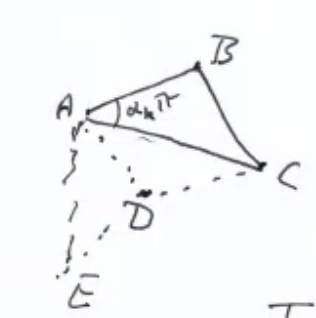
\includegraphics[scale=0.5]{triangle.png}
\end{center}
If we let $B$ reflect to $D$ in $AC$, then the extension of $g$ to $ADC$ will also take real values on $AD$ and $DC$.  Also, the exnteded $g$ will extend by reflection to $ADE$.  The result of the reflection in $AC$ and $AD$ is a rotation by $2 \phi + \psi$, where $\phi + \psi = \alpha_k \pi$, so a rotation by $2 \alpha_k \pi$ and when we preform $2$ reflections, there is no more conjugation of the function.  
\end{document}
